%%%%%%%%%%%%%%%%%%%%%%%%%%%%%%%%%%%%%%
% Multiplicative domain poster
% Created by Nathaniel Johnston
% August 2009
% http://www.nathanieljohnston.com/2009/08/latex-poster-template/
%%%%%%%%%%%%%%%%%%%%%%%%%%%%%%%%%%%%%%

\documentclass[final]{beamer}
\usepackage[scale=1.2]{beamerposter}
\usepackage{graphicx}			% allows us to import images
\usepackage{fancyvrb}
\usepackage{algorithm}
\usepackage{algorithmic}
\usepackage{listings}
\lstset{language=Matlab}
\lstset{basicstyle=\footnotesize\ttfamily,breaklines=true}
\lstset{framextopmargin=10pt,frame=single}
%-----------------------------------------------------------
% Custom commands that I use frequently
%-----------------------------------------------------------

\newcommand{\bb}[1]{\mathbb{#1}}
\newcommand{\cl}[1]{\mathcal{#1}}
\newcommand{\fA}{\mathfrak{A}}
\newcommand{\fB}{\mathfrak{B}}
\newcommand{\Tr}{{\rm Tr}}
\newtheorem{thm}{Theorem}

%-----------------------------------------------------------
% Define the column width and poster size
% To set effective sepwid, onecolwid and twocolwid values, first choose how many columns you want and how much separation you want between columns
% The separation I chose is 0.024 and I want 4 columns
% Then set onecolwid to be (1-(4+1)*0.024)/4 = 0.22
% Set twocolwid to be 2*onecolwid + sepwid = 0.464
%-----------------------------------------------------------

\newlength{\sepwid}
\newlength{\onecolwid}
\newlength{\twocolwid}
\setlength{\paperwidth}{46.81in}
\setlength{\paperheight}{33.11in}
\setlength{\sepwid}{0.024\paperwidth}
\setlength{\onecolwid}{0.22\paperwidth}
\setlength{\twocolwid}{0.464\paperwidth}
\setlength{\topmargin}{-1in}
\usetheme{confposter}
\usepackage{exscale}

%-----------------------------------------------------------
% The next part fixes a problem with figure numbering. Thanks Nishan!
% When including a figure in your poster, be sure that the commands are typed in the following order:
% \begin{figure}
% \includegraphics[...]{...}
% \caption{...}
% \end{figure}
% That is, put the \caption after the \includegraphics
%-----------------------------------------------------------

\usecaptiontemplate{
\small
\structure{\insertcaptionname~\insertcaptionnumber:}
\insertcaption}

%-----------------------------------------------------------
% Define colours (see beamerthemeconfposter.sty to change these colour definitions)
%-----------------------------------------------------------

\setbeamercolor{block title}{fg=ngreen,bg=white}
\setbeamercolor{block body}{fg=black,bg=white}
\setbeamercolor{block alerted title}{fg=white,bg=dblue!70}
\setbeamercolor{block alerted body}{fg=black,bg=dblue!10}

%-----------------------------------------------------------
% Name and authors of poster/paper/research
%-----------------------------------------------------------

\title{Optimal Waterfilling Policy for Energy Harvesting Wireless Networks}
\author{Sasank Chilamkurthy; Advisor: Prof. Abhay Karandikar}
\institute{Department of Electrical Engineering, Indian Institute of Technology Bombay}

%-----------------------------------------------------------
% Start the poster itself
%-----------------------------------------------------------
% The \rmfamily command is used frequently throughout the poster to force a serif font to be used for the body text
% Serif font is better for small text, sans-serif font is better for headers (for readability reasons)
%-----------------------------------------------------------

\begin{document}
\begin{frame}[t]
  \begin{columns}[t]												% the [t] option aligns the column's content at the top
    \begin{column}{\sepwid}\end{column}			% empty spacer column
    \begin{column}{\onecolwid}
      \begin{alertblock}{The Big Question}
        \rmfamily{For energy harvesting transmitter, how do we allocate power for slots to maximise throughput?}
      \end{alertblock}
      \vskip2ex
      \begin{block}{What is WaterFilling Policy}
\rmfamily{It is a optimal power allocation scheme if we have $k$ independent Gaussian channels with different noise levels in parallel with common power constraint $\bar{P}$. 
This is a model for fading channel for $k$ time slots each having independent fading states.
\begin{figure}
	\begin{center}
		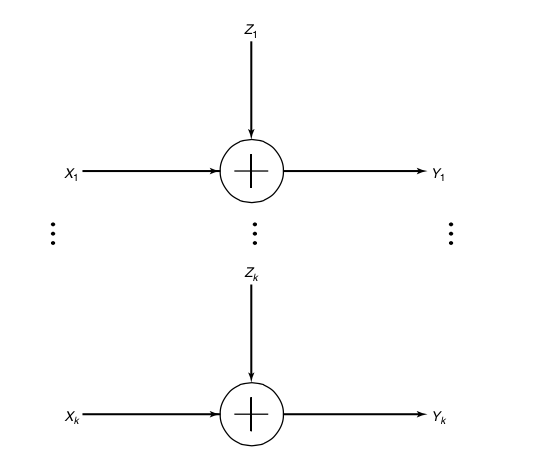
\includegraphics[width=8in]{parallelchannels}
		\caption{Parallel Gaussian Channels}
	\end{center}
\end{figure}
        
\begin{itemize}
	\item If we allocate a power $P_i$ to $i$th channel which has AWGN noise level of $N_i$, 
	Then the capacity of $i$th channel is \[R_i = 1/2\log(1 + P_i/N_i)\] 
	\item Average Power over $k$ channels is constrained by $P$. i.e, $ \frac{\sum_i{P_i}}{k} \leq \bar{P} $
	\item We want to maximize $\sum_i R_i$ subject to constraints $\sum_i{P_i} \leq k\bar{P}$ and $P_i \geq 0$ 			
	\item This can be solved by Lagrangian multipliers. Solution of this optimization problem turns out to be 
	\[ P_i = (\nu - N_i)^+\]
	where $f^+ = \max(f,0)$ and $\nu$ is chosen such that $\sum_i (\nu - N_i)^+ = P_i$. This $\nu$ is called \emph{Water Level}.
	\item If $i$th channel corresponds to $i$th fading state with fading coefficient $F_i$, then $N_i = N/F_i^2$ where 
	$N$ is SNR of the channel when fading coefficient is $1$.

\end{itemize}
}
      \end{block}
    \end{column}

    \begin{column}{\sepwid}\end{column}			% empty spacer column
    \begin{column}{\twocolwid}							% create a two-column-wide column and then we will split it up later
      \begin{columns}[t,totalwidth=\twocolwid]	% split up that two-column-wide column
        \begin{column}{\onecolwid}\vspace{-.69in}

				\begin{block}{What is a Energy Harvesting Wireless Network}
					\rmfamily{This is modeled as standard fading channel \[Y_i = F_iX_i + N_i\] with the following extra conditions
					\vspace{0.1in}
					\begin{itemize}\justifying	% the \justifying command forces the items in the list to have full justification (they don't by default)
						\item Transmitter Node has a rechargable battery. It gets recharged using energy harvested from the sorroundings. It has a maximum capacity $E_{max}$
						\item Ammount of battery recharge is not known before hand and varies randomly due to environmental fluctuations
						\item Suppose in $i$th slot, $E_i$ is energy available in the battery, $P_i$ is energy consumed for transmission and $K_i$ is recharge from the harvesting,
						\[ E_{i+1} = \min(E_i - P_i + K_i,E_{max}) \]
						\item $K_i$ is iid random variables which can be modelled to depend on current battery charge. 
						We used $K_i = U_i(1 - e^{\alpha(E_n - E_{max}) })$ where $U_i$ is a uniform random variable. 
						\item Note that $P_i$ has to be at most $E_i$. This is what makes power allocation harder. If $i$th slot is really good and if we do not have enough energy in the battery, we'll have to use suboptimal power for transmission.
						\item We assume that transmitter has full CSI at $i$th slot and it has both channel fading characteristics and recharge characteristics available.
					\end{itemize}}
				\end{block}
			\end{column}


        \begin{column}{\onecolwid}\vspace{-.69in}
          \begin{block}{Simulation Results}
            \rmfamily{
				\begin{figure}[H]
				\centering
				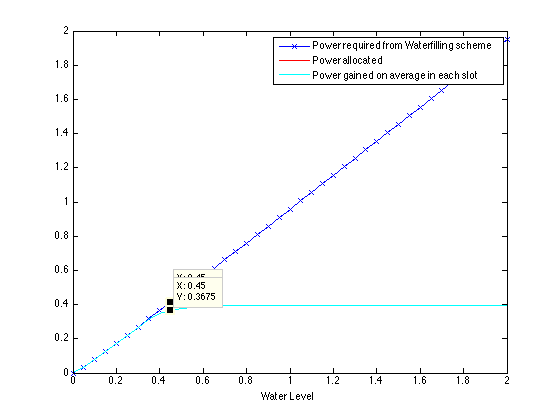
\includegraphics [width=9.5in]{AverageSimulation_01.png}
				\caption{Expected power values of different quantities vs. \texttt{waterlevel} ($\nu$)}
				\label{fig:1}
				\end{figure}
				
				\begin{figure}[H]
				\centering
				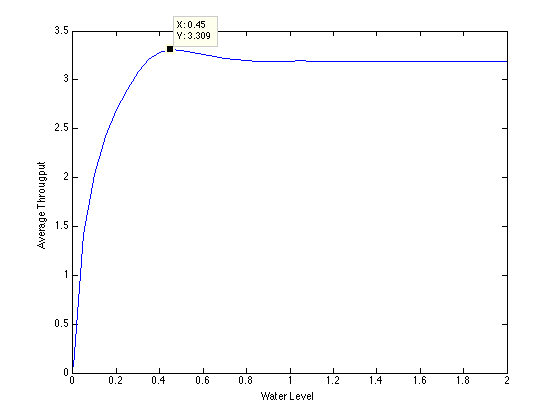
\includegraphics [width=9.5in]{AverageSimulation_02.png}
				\caption[fig2]{Expected throughput for a given \texttt{waterlevel} ($\nu$)}
				\end{figure}
			}	
          \end{block}
        \end{column}
      \end{columns}
      %\vskip2.5ex
		\begin{alertblock}{Our Problem}		% an ACTUAL two-column-wide column
			\rmfamily{Suppose that the an energy harvesting tranmitter node has full CSI, energy recharge characterstics and fading state characterstics available, which water level of the waterfilling policy does it have to chose to maximise average expected throughput 
			$1/N\sum_i^N \bb{E}[\log(1 + P_iF_i^2/N_0)]$ }
		\end{alertblock}

      \begin{columns}[t,totalwidth=\twocolwid]
        \begin{column}{\onecolwid}
        \begin{block}{Simulation Methodolgy}
          \rmfamily{
          \begin{itemize}\justifying
            \item For each waterlevel $\nu$, $N$ slots will be simulated. 
            \item $t$ such independent sample paths for system are generated and are averaged.
				This is an approximation for expected value over randomness involved in battery rechanrge.
          \end{itemize}}
        \end{block}
      \end{column}
      \begin{column}{\onecolwid}


        \begin{block}{\fontsize{1.5cm}{0.8em}\selectfont Infinitesimal Perturbation Analysis}
          \rmfamily{
To maximize R, we do independent simulations of the system, {\small $\hat{X}_1,\hat{X}_2 \dots, \hat{X}_N$} and {\small $\mathring{X}_1,\mathring{X}_2 \dots, \mathring{X}_N$} corresponding to {\small$\nu(n)+\delta/2$} and {\small $\nu(n) - \delta/2$} and perform the iterate
{
\small
\[\nu(n+1) = \nu(n) - a(n)\left(\frac{R(\hat{X}_1,\hat{X}_2 \dots, \hat{X}_N) - R(\mathring{X}_1,\mathring{X}_2 \dots, \mathring{X}_N)}{\delta} \right) \]
}
}
        \end{block}

      \end{column}
    \end{columns}
  \end{column}
  \begin{column}{\sepwid}\end{column}			% empty spacer column
  \begin{column}{\onecolwid}

    \begin{block}{Algorithm to Find Best Waterfilling Scheme}
\rmfamily{

We use \emph{Infinitesimal Perturbation Analysis (IPA)} scheme to find optimal waterlevel $\nu$.
\medskip

To increase stability of the algorithm, we simulate chain \texttt{times} number of times and take average gradient. 
\vskip2.5ex
\lstinputlisting{src.m}
}

This algorithm gives following results when parameters from Figure 3 are used:
\vskip2.5ex
\lstinputlisting{results.txt}


    \end{block}

    \begin{block}{Future Work}
      \rmfamily{
			Although running of the algorithm has been verified by simulations, 
			to theoretically prove the convergence of the above algorithm we need to prove the quasi-concaveness of expected average throughput.
			This is being worked on.
		}
    \end{block}
  \end{column}
  \begin{column}{\sepwid}\end{column}			% empty spacer column
 \end{columns}

\end{frame}
\end{document}
